\documentclass[12pt]{article}

\usepackage{amsfonts}
\usepackage{graphicx}
\usepackage{float}
\usepackage{titling}
\usepackage{amsmath} 
\usepackage{amssymb}
\usepackage{subfigure}
\usepackage[colorlinks=true, urlcolor=blue, linkcolor=blue]{hyperref}

\setlength{\droptitle}{-10em} 
\addtolength{\oddsidemargin}{-.875in}
\addtolength{\evensidemargin}{-.875in}
\addtolength{\textwidth}{1.75in}
%\addtolength{\textheight}{1.75in}
\makeatletter
\def\ps@pprintTitle{%
\let\@oddhead\@empty
\let\@evenhead\@empty
\def\@oddfoot{}%
\let\@evenfoot\@oddfot}
\makeatother


\begin{document}
	\title{A Network Perspective on LDA *DRAFT*}
	\author{Cindy Cook \\ \normalsize Network Analysis Final Project \\ \normalsize 5 May 2016}
	\date{}
	\maketitle

\section{Introduction}

With an increase in the amount of digitized text, topic modeling has become an important area of research. One of the most popular methods for topic modeling is Latent Dirichlet Allocation (LDA) first described in \cite{lda}. LDA, a probabilistic hierarchical generative model, uses the Bayesian framework to discover hidden structure, or \textit{topics},  within a set of documents referred to as a corpus. Given a document, the distribution of latent topics is found through estimation of the posterior distribution. However, this is very challenging and computationally demanding since the posterior distribution of the latent variables given a document is intractable. A heavy development of fast and accurate approximation methods applied to LDA have been developed providing a user with several estimation options. A few of these options include collapsed Gibbs sampling (CGS) \cite{CGS}, collapsed variational Bayesian inference \cite{CVB}, maximum likelihood estimation \cite{ML}, and maximum a posteriori estimation \cite{MAP}. In \cite{lda}, a variational EM (VEM) algorithm is applied to solve the problem. Although the development of these methods have allowed researchers to get answers, a major problem lies in the fact that using different methods can often lead to conflicting results.
\\
\\
There have been several studies published comparing estimation procedures for LDA including \cite{BleiComp}, \cite{Comp}, \cite{CVB}, and \cite{Comp2}. Most comparison studies focus on a single corpus and evaluate different estimation methods using precision/recall statistics. In general, these papers offer good advice, but do not address the main problem of identifying inaccurate results. More recently, deeper theoretical problems with LDA have been highlighted by Lancichinetti in \cite{main}. The paper ``High-Reproducibility and High-Accuracy Method for Automated Topic Classification" shows that the likelihood of the true generating model can be smaller then the likelihood of alternative models in the LDA framework \cite{main}. After demonstrating their theoretical concerns, the authors tweak the LDA algorithm to provide a process they call TopicMapping, which leads to more robust results. TopicMapping involves five stages. The first is to clean the corpus, which involves stemming and removing of stop words. The second stage is to project the term frequency matrix onto the word space. The third stage filters the edges according to a Poisson distribution. The fourth stage is to apply InfoMap clustering to obtain starting values for each topic distribution over the words. The fifth and final stage is to apply LDA with these initial starting values. This process decreases the size of the parameter space, which aids in the estimation procedure. TopicMapping is tested on both simulated and real world corpus's.    
\\
\\
Although TopicMapping appears to solve the basic problems involved when applying LDA, I will show that it fails to produce both accurate and reproducible results across all types of corpus's. I hypothesis that basic differences in the modularity of the projected word network of a corpus determines whether or not TopicMapping will outperform LDA. The second section of this paper goes through a replication study done to ensure that the results of TopicMapping published in \cite{main} are accurate. It is also performed to make sure that I have the proper code and algorithms in place to apply their methods to other datasets. The third section introduces a new data set and explains how the networks used in this paper were obtained. The fourth section first applies TopicMapping to the new data and obtains neither accurate nor reproducible results. It then compares both the new and original corpus's using descriptive statistics. The fifth section uses ERGMs to analyze the differences between the two networks. The sixtha nd final section concludes the paper with a discussion of the results and future directions.

\section{Replicate the Study}

The paper, ``High-Reproducibility and High-Accuracy Method for Automated Topic Classification," consists of four main parts \cite{main}. The first points out a major limitation to the LDA algorithm developed by Blei as a topic model \cite{lda}. The second describes a new method called TopicMapping developed to overcome theoretical drawbacks of LDA. The third consists of comparing the accuracy and reproducibility of TopicMapping as compared to LDA and pLSA \cite{plsa} on synthetic data. The final aspect of the paper, applies TopicMapping to two real world datasets. I have been able to successfully reproduce the accuracy and reproducibility results for the comparisons between TopicMapping and randomly seeded LDA in both the simulated studies and one of the real world applications. The results of my replication can be found in \hyperlink{A}{Appendix A}. All data and scripts can be found on github:   \href{https://github.com/cmcook22/Cook_Networks_Project}{here} .    

\section{The Data}

There are two main `real world' datasets used to test the TopicMapping algorithm:  Science and Wikipedia. The Science corpus contains $28,838$ documents from the web of science, where each document contains the title and abstract of a paper published in one of six top journals from different disciplines. After preprocessing the data, there are $106,143$ unique words and over $8.7 \times 10^{6}$ edges. The Wikipedia dataset contains over $4 \times 10^{6}$ nodes with over $800 \times 10^{6}$ edges. Due to the size of the Wikipedia data set, I was unable to receive this information from the authors of \cite{main}. Therefore, I focused my replication and extension on the Science data set only. Although the Science corpus was easily sent to me, it is still considered `large.' In R, the adjacency matrix is too large to be stored. 
\\
\\
Due to the size of the WoS dataset, I randomly selected $10$ documents in each subject to create a working dataset for a total of $60$ documents. This dataset is referred to as the Science corpus. The second corpus I will be considering was obtained from Indeed.com. Each document contains the past work experience from resumes within five different fields: teaching, graphic design, architecture, nursing, and accounting. The corpus contains $50$ documents. I will refer to this corpus as the Indeed corpus. 

\subsection{Creating the Networks}

After obtaining documents for both corpus's, a network of words is created in R by first using the \textit{tm} package to obtain the term frequency matrix. Then a stemmer is applied, and basic English stop words are removed. The stemmer and stop words applied are the same as used in \cite{main}. The \textit{bipartite} package is then used to project this term frequency (i.e. the adjacency matrix for a two-mode network) onto a one-mode network of words weighted by the number of times a pair of words appears together across all documents. Then the filtering process laid out in \cite{mainExtra} is applied. The following shows the size of each network through this process:
\vspace{2mm}
\begin{center}
	\begin{tabular}{ |c|c|c||c|c|  }
		\hline
		&Science& &Indeed &\\
		\hline
		&Nodes&Edges&Nodes&Edges \\
		\hline
		original corpus& 2189& &1717 & \\
		cleaned corpus& 1995& & 1092&\\
		projected network& 1995& 121440& 1092&50534\\
		filtered network& 1995&121039 & 1092&50186\\
		\hline
	\end{tabular}
\end{center}
\vspace{2mm}
Plotting the networks using the Fruchterman-Reingold layout in NodeXL we obtain the following images: 
\vspace{2mm}
\begin{figure}[H]
	\centering
	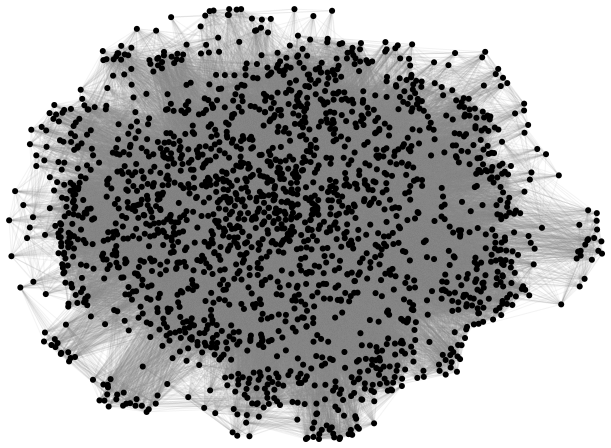
\includegraphics[scale=0.5]{Images/Sci.png}
	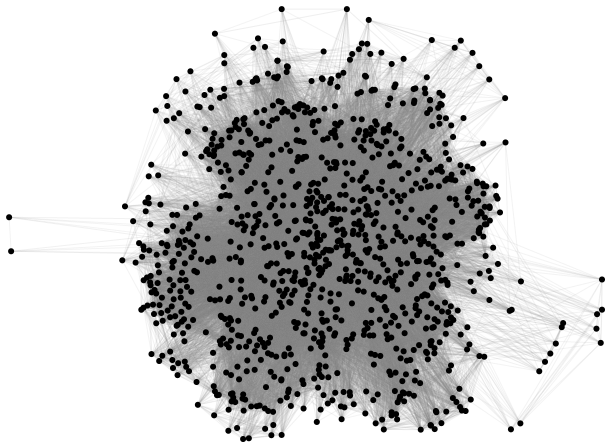
\includegraphics[scale=0.5]{Images/Ind.png}
	\caption{on the left:  Science word network; on the right:  Indeed word network}
\end{figure}
In both networks, we can see black filled in circles, which are words that appear equally in all topics and are not assigned a clustering id. There are six and five clusters, one for each topic in Science and Indeed, respectively. InfoMap perfectly assigns one topic shown as the green open circles, but does not perfectly assign topics in any other cluster, but these are the only results we can conclude from visual analysis.

\section{Comparison}

Using the code provided to me, I run TopicMapping on both Science and Indeed $300$ times:  $100$ times with $K=3$, $100$ times with $K=6$, and $100$ times with $K=10$. I also run the LDA function in R with the VEM method for estimation and different starting seeds on both Science and Indeed $300$ times$100$ times with $K=3$, $100$ times with $K=5$, and $100$ times with $K=10$. Note that for Science and Indeed the correct number of toopics is $5, 6,$ respectively. To compare results, I calculate the accuracy and reproducibility as defined in \cite{mainExtra}. I obtained the following results: 
\vspace{2mm}
\begin{figure}[H]
	\centering
	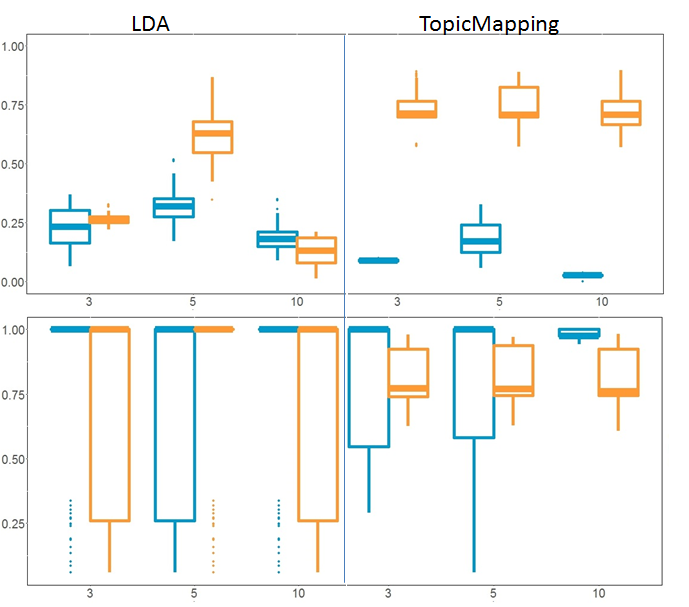
\includegraphics[scale=0.5]{Images/results.png}
	\caption{Plots on the top show boxplots of the accuracy for 100 runs on Science(orange) and Indeed (blue). Plots on the bottom show the reproducibility for the 100 runs.}
\end{figure}
\vspace{2mm} 

\noindent We can see that TopicMapping performed with approximately $75\%$ accuracy and $80\%$ reproducibility for the Science corpus. However, the accuracy is around $10\%$ and the reproducibility is extremely variable for the Indeed corpus. We should also notice that TopicMapping outperforms LDA only on the Science corpus, but fails to produce better results for the Indeed corpus. I hypothesize that TopicMapping is highly dependent on the clustering done through InfoMap. If InfoMap does not produce accurate results, it can lead the estimation procedure of LDA into the wrong part of the parameter space resulting in completely inaccurate results. The major difference between the two corpus's lies in the fact that words used in titles and abstracts of journal articles do not readily appear across different disciplines. Whereas words used in resumes to describe past work experience cross fields more easily. In fact, we can see from the following plot, the proportion of words from our two cleaned corpus's that cross these boundaries:
\vspace{2mm}
\begin{figure}[H]
	\centering
	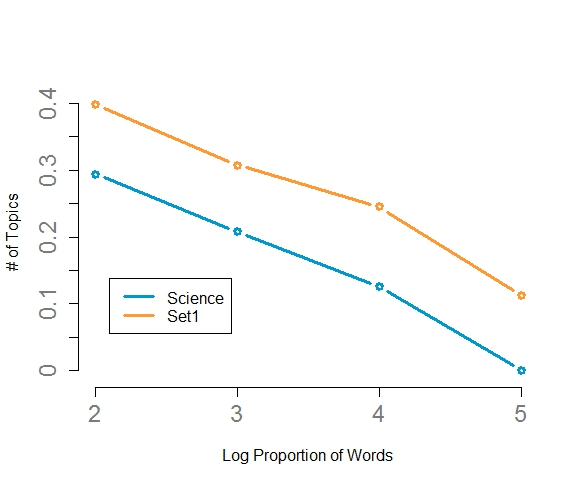
\includegraphics[scale=0.5]{Images/props.jpeg}
\caption{The proportion of unique words in each corpus that belong to at least 1, 2, 3, 4, and 5 topics for both the Science (orange) and Indeed (blue) corpus's are shown above.}
\end{figure}
\vspace{2mm}

\noindent We can clearly see that close to zero percent of the Science corpus unique words are shared across all six topics, whereas, close to $20\%$ of the unique words in the Indeed corpus are shared across all job categories.

\subsection{Descriptive Statistics}

To begin analysis on these networks, I use the \textit{igraph} package in R to measure the betweenness centrality for each node, which will allow me to analyze structural holes and bridges. Words that are highly used within each document and common across all documents will have high betweenness scores: 
\vspace{2mm}
\begin{figure}[H]
	\hfill
	\subfigure[Science]{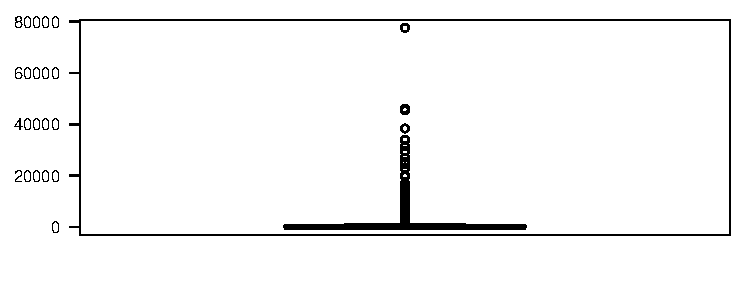
\includegraphics[scale=0.5]{Images/Sci_between.pdf}}
	\hfill
	\subfigure[Indeed]{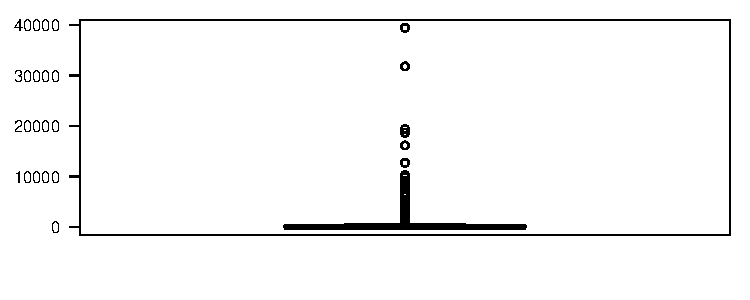
\includegraphics[scale=0.5]{Images/Indeed_between.pdf}}
	\hfill
	\caption{Boxplots of the betweenness centrality scores for each corpus.}
\end{figure}
\vspace{2mm}

\noindent Words with the highest betweenness scores for Science are as follows:  result (123287.95), use (67756.22), model (67159.62), data (60749.09), suggest (56224.20), and studi (55947.48). Words with the highest betweenness scores for Indeed are as follows:  present (39422.6), pa (31815.2), respons (19401.64), includ (18680.75), work (16158.91), and design (12703.92). As predicted, these words are used often in each document no matter what discipline or field the document is in. This fact would be obvious for any projected word network. There is only a slight difference in the distribution of betweenness scores. We find that for the Science corpus only $680$ words in the network, or about $(34\%)$, have a betweenness centrality greater than one, while $1829$, or about $(92\%)$, have a betweenness score greater than $0$. For the Indeed corpus. For the Indeed corpus, $404$ words, or about $(37\%)$ of the words, have a betweenness score greater then 1, while $1061$, or about $(98\%)$ of the words, have a betweenness score greater than 0. I would expect this difference to be more pronounced given the TopicMapping results. 
\\
\\
Next, I will find the transitivity score of the network. Transitivity can be used as a clustering coefficient for networks. Thus, I hypothesis that this value is positive for both networks, but higher for the Science corpus than the Indeed corpus. However, it turns out that this measure it similar for both corpus:  $0.4181239$ for the Science corpus and $0.4279717$ for the Indeed corpus. Taking a closer look, we see the following triad censuses:
\vspace{2mm}
\begin{center}
	\begin{tabular}{ |c||c|c|c|c|  }
		\hline
		&003&102&201&300 \\ 
		\hline 
		Science& $83.40\%$ & $15.21\%$ & $1.12\%$ & $0.27\%$ \\
		Indeed& $77.78\%$ & $19.67\%$ & $2.04\%$ & $0.51\%$ \\
		\hline
	\end{tabular}
\end{center}
\vspace{2mm}

\noindent Since both networks are undirected, there are only four possible triads, and the distribution of these are very similar in both Science and Indeed. In fact, it turns out that several descriptive statistics are very similar for both networks including density $(0.06085374, 0.08424908)$, degree assortitivity, $(-0.06119152, -0.12577)$, and their degree distributions:
\vspace{2mm}
\begin{figure}[H]
	\centering
	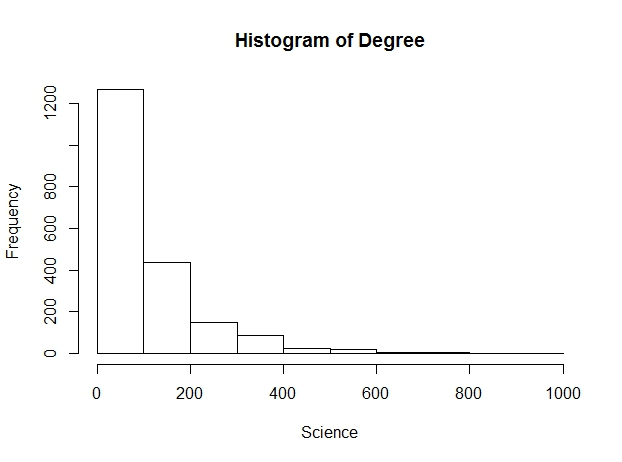
\includegraphics[scale=0.4]{Images/degree_hist_sci.jpeg}
	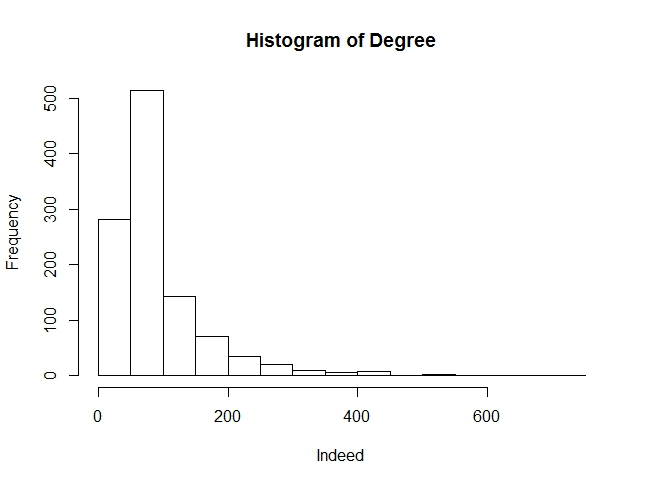
\includegraphics[scale=0.4]{Images/degree_hist_ind.jpeg}
	%\caption{.}
\end{figure}
\vspace{2mm} 

\noindent as well as their modularity for several different methods:
\vspace{2mm}
\begin{center}
	\begin{tabular}{ |c|c|c|  }
		\hline
		&Modularity& \\
		\hline
		Clustering Type&Science&Indeed \\ 
		\hline 
		InfoMap& 0.3884&0.3881 \\
		Fast-Greedy& 0.3398& 0.3358\\
		Eigenvalue& 0.3624&0.3616 \\
		Louvain&0.3936&0.3904 \\
		Walktrap&0.3257&0.3431 \\
		\hline
	\end{tabular}
\end{center}
\vspace{2mm}
\noindent TopicMapping uses the InfoMap clustering algorithm, which yields $41$ different clusters for the Science Corpus and $24$ for the Indeed corpus. Plotting the networks with nodes colored according to InfoMap cluster, we obtain the following:
\vspace{2mm}
\begin{figure}[H]
	\centering
	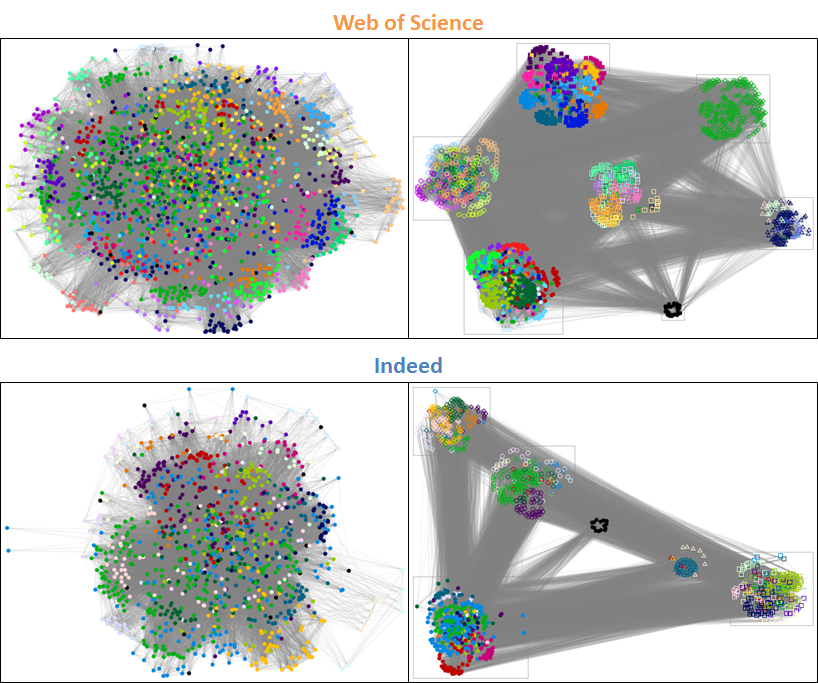
\includegraphics[scale=0.5]{Images/networks.png}
	\caption{Science is plotted on the top, while Indeed is plotted on the bottom. The network colored according to InfoMap clusters is on the left, while words are clustered and are assigned symbols according to the topic they appear in the most often through the corpus.}
\end{figure}
\vspace{2mm}

\section{ERGMS}

I hypothesize that projected word networks which do not cluster well will not perform well in terms of TopicMapping. Since there do not appear to be any differences in the word networks from a structural stand-point, I plan to explore the extent of homophily in each network as quantified using ERGMS. For each network, I first use the InfoMap clustering algorithm in the \textit{iGraph} package in R to obtain membership ids for each word. I then fit an ergm with the nodematch term to test for homophily in each network. I include both edges and isolates as controls. Although there are several clustering algorithms to choose from, I focus only on InfoMap because it is used in the TopicMapping algorithm. The coefficients were obtained using MLE. The MCMC diagnostic plots as well as goodness of fit plots can be found in \hyperlink{B}{Appendix B}. I obtain the following Maximum Pseudolikelihood Results:
\vspace{2mm}
\begin{center}
	\begin{tabular}{ |c|c|c|c|c||c|c|c|c|c|c|  }
		\hline
		&Science&&&&Indeed&&& \\
		\hline
		&Estimate&Std. Error&MCMC$\%$&p-value&Estimate&Std. Error&MCMC$\%$&p-value \\ 
		\hline 
		edges&-3.3591&0.0040&0&$<0.0001$&-2.9925&0.0063&0&$<0.0001$\\
		isolate&-Inf&0&0&$<0.0001$&-Inf&0&0&$<0.0001$\\
		homophily&3.3696&0.0077&1&$<0.0001$&3.3616&0.0122&0&$<0.0001$\\
		\hline
	\end{tabular}
\end{center}
\vspace{2mm}
First note that the coefficient for the isolates term is negative infinity since there are no isolates in either network. I included the term because by definition, there should never be any isolate in a word projection network. Next we should notice that both of the homophily terms are significant, positive, and approximately $3.36$. There is an extremely slight decrease in the term for Indeed, but not as much as I expected. 
\\
\\
It is important before analyzing these results further to take a close look at the goodness of fit statistics. We can clearly see that neither ergm fits well. After several attempts to obtain a better fit by including terms for different degree properties, edge weights, and several other options, none of the more complex models converged. It is important to verify these results. I will first apply QAP regression, where the response is the weighted projected word network, and the predictor is the binary network indicating if two nodes are connected and if they are in the same cluster. I use the netlm function in the sna package in R. I obtain the following results:
\vspace{2mm}
\begin{center}
	\begin{tabular}{ |c|c|c|c|c||c|c|c|c|  }
		\hline
		&Science&&&&Indeed&&& \\
		\hline
		&Estimate&Pr$(\le b)$ &Pr$(\ge b)$ &Pr$(\ge |b|)$&Estimate&Pr$(\le b)$ &Pr$(\ge b)$ &Pr$(\ge |b|)$ \\ 
		\hline 
		intercept&0.0463& 1&   0&  0&0.0621& 1&       0&       0      \\
		Homophily&0.9537 &1  &0   &0&0.9379 &1       &0       &0\\
		\hline
		Adj. $R^{2}$&0.2406&&&&0.245&&& \\
		\hline
	\end{tabular}
\end{center}
\vspace{2mm}
Note that for the binary predictor, a one represents that two words are tied and in the same cluster. As we can see, the two models are extremely similar, which is expected after seeing the ergm output. The coefficients have the same sign, but are lower. The models do have the same interpretation:  a new additional node with a cluster id will attach to other nodes with the same clustering id with a coefficient of about 0.9 on average and will attach to a node with different clustering ids with a coefficient of about 0.05 regardless of corpus. These results suggest that there is positive homophily in both networks at a similar rate, which is contrary to what I hypothesized.   
\\
\\
As a second precaution, I will perform a conditional uniform graph test to make sure that the clustering coefficient is in fact significantly different for both models as compared to what would be expected based on each network's respective dyad distribution. I use the rguman function in the sna package to simulate 100 random netwroks conditional on the dyad distribution for each corpus. I then obtain the clustering ids from the InfoMap algorithm and calculate the modularity for each simulated network. Comparing these results, it is easy to see that for all of the simulated networks, the modularity is negative and close to $0$. Where as we saw earlier, the modularity for both Science and Indeed was close to $0.39.$ 
 
\section{Conclusions}





\newpage
\begin{thebibliography}{4}
		
	\bibitem{STACK}
	Anonymous. (2012),
	``Two R Packages for Topic Modeling, lda and topicmodels?" \textit{Cross Validated}: http://stats.stackexchange.com/questions/24441/two-r-packages-for-topic-modeling-lda-and-topicmodels.
	
	\bibitem{Comp} 
	Asuncion, A., Welling, M., Smyth, P., and Teh, Y.  (2009),
	``On Smoothing and Inference for Topic Models." 
	\textit{UAI}: 27-34.
	
	\bibitem{plsa}
	BHoffman, T.  (1999),
	``Probabilistic Latent Semantic Indexing."
	\textit{Proccedings of the Twenty-Second Annual International SIGIR Conferance}.
		
	\bibitem{lda}
	Blei, D., Ng, A., and Jordan, M.  (2003),
	``Latent Dirichlet Allocation."
	\textit{Journal of Machine Learning Research}: 3 993-1022.
	
	\bibitem{Ccode}
	Blei, D. (2004),``LDA-C."
		
	\bibitem{ldaR}
	Chang, J.  (2015),
	``Package `lda'."
	\textit{CRAN}.

	\bibitem{MAP}
	Chien, J., and Wu, M.  (2008),
	``Adaptive Bayesian Semantic Analysis."
	\textit{Audio, Speech, and Language Processing}, IEEE Transactions on: 16(1), 198-207.

	\bibitem{CGS}
	Griffiths, L. and Steyvers, M.  (2004),
	``Finding Scientific Topics."
	\textit{PNAS}: 1(Suppl 1), 5228-5235.

	\bibitem{topicsR}
	Grun, B. and Hornik, K.  (2015),
	``Package `topicmodels'."
	\textit{CRAN}.
	
	\bibitem{ML}
	Hofmann, T.  (2001),
	``Unsupervised Learning by probabilistic Latent Semantic Analysis."
	\textit{Machine Learning}: 42(1), 177-196.
	
	\bibitem{main}
	Lancichinetti, A., Sirer, M., Wang, J., Acuna, D., Kording, K., and Amaral, Luis. (2015),
	``High-Reproducibility and High-Accuracy Method for Automated Topic Classification."
	\textit{Physical Review X}: 5, 0011007, 2160-3308.
	
	\bibitem{mainExtra}
	Lancichinetti, A., Sirer, M., Wang, J., Acuna, D., Kording, K., and Amaral, Luis. (2015),
	``High-Reproducibility and High-Accuracy Method for Automated Topic Classification: Supplemental Material."
	\textit{Physical Review X}: 5, 0011007, 2160-3308.
	
	\bibitem{BleiComp} 
	Mukherjee, I. and Blei, D.  (2009),
	``Relative Performance Grantees for Approximate Inference in Latent Dirichlet Allocation." 
	\textit{NIPS}: 21, 1129–1136.
	
	\bibitem{Comp2}
	Speh, J., Muhic, A., and Rupnik, J.  (2013),
	``Parameter Estimation for Latent Dirichlet Allocation." \textit{Artificial Intelligence Laboratory}: Ljubljana, Slovenia.
		
	\bibitem{CVB}
	Teh, Y. W., Newman, D., and Welling, M.  (2007),
	``A Collapsed Variational Bayesian Inference Algorithm for Latent Dirichlet 
	Allocation."\textit{NIPS}: 3, 1353-1360.
	
\end{thebibliography}

\newpage
\appendix
\hypertarget{A}{}
\section{Replication Study}
\subsection{LDA Limitations}
The paper \cite{main} begins with a simple thought experiment. Given a Corpus consisting of documents in three distinct languages, say English, Spanish, and French, let all words in each language be unique and each document contain only one language. Ideally, a topic model would produce three distinct topics, one for each of the unique languages. However, this is not the case with LDA. The authors of \cite{main} show the likelihood of the generative model (i.e. placing all English documents in one topic, all Spanish documents in another, and all French documents in the last topic) is not always maximum. In fact they describe an alternative model, which theoretically obtains a higher likelihood. The alternative model is defined by separating one language into two dialect topics and combining the other two languages into one topic. In fact the authors prove in the supplemental material that, ``it is possible to find an extremely large number of alternative models (with the same number of topics) which overfit some topics and underfit some others but have a better likelihood then the true generative model" \cite{mainExtra}. These results are visualized in Fig. 2 (pg. 3,\cite{main}). Part a illustrates the differences in the generative and alternative models considered. Part b and c show the theoretical limits on the log likelihood for both generative and alternative models when considering a vocabulary of $60$ unique words, where $20$ are in either $E, S,$ or $F$. The corpus contains $1000$ documents, where each document contains $10$ words chosen uniformly from one language. Specifically, they show that the for these particular parameter values, if the fraction of $E$ documents in the corpus is greater than $0.936,$ then the likelihood of the alternative model become greater than the likelihood for the generative model. 
\\

\noindent In order to replicate part d of Fig. 2, I will first create a synthetic language corpus and then apply the LDA algorithm as programed in the \textit{topicmodels} package in R. We can determine the success rate as shown in Fig. 2 (pg. 3 \cite{main}) part d. Here, I also consider the average cosine similarity between each document's topic distribution and the true topic distribution. Following the process in \cite{main}, I first create a list of twenty words in English $E$, Spanish $S$, and French $F$. I then create a corpus of $1000$ documents, where the number of $E, S,$ and $F$ documents follow the following equation:
$$
100=pE+\frac{(100-p)}{2}S+\frac{(100-p)}{2}F,
$$ 
for $p=0.5, 0.6, 0.7, 0.8, 0.9, 0.96$. Note that each of the twenty words of a particular language has an equal probability of being sampled for each document with replacement, and each document consists of exactly ten words. I then apply LDA using the Variational EM Approach, which was used in \cite{main}. I run the algorithm $100$ times calculating the average cosine similarity and success rate with each run to obtain the following results:   
\vspace{2mm}
\begin{center}
	\begin{tabular}{ ||c|c|c|c|c|c|c||  }
		\hline
		$p$ &0.5&0.6&0.7&0.8&0.9&0.96 \\ 
		\hline 
		Min.    &0.5763 &0.5593 &0.5318 &0.5780 &0.5774 &0.5765\\
		1st Qu. &0.5844 &0.5821 &0.5802 &0.5800 &0.5791 &0.5774\\
		Median  &1.0000 &0.5871 &0.5834 &0.5822 &0.5802 &0.5777\\
		Mean    &0.8252 &0.7240 &0.6481 &0.5919 &0.5803 &0.5776\\
		3rd Qu. &1.0000 &1.0000 &0.5913 &0.5852 &0.5809 &0.5779\\
		Max.    &1.0000 &1.0000 &1.0000 &1.0000 &0.5858 &0.5783\\
		\hline
	\end{tabular}
\end{center}
\vspace{2mm}

\noindent We Notice that the minimum cosine similarity stays relatively constant across percent levels. This is due to the fact that in all runs, there are only three options of outcomes:  First, LDA correctly identifies the generative model resulting in a cosine similarity measure of about $0.99$; Second, LDA identifies the alternative model resulting in a cosine similarity of about $0.73$; and Third, LDA assigns a uniform topic distribution for each document resulting in a cosine similarity of about $0.55$. Although LDA applies a uniform topic distribution each of the corpuses at least once, we notice that when the percent level is $0.9$ and $0.96$ the algorithm applies a uniform topic distribution in all $100$ runs. Also, notice that the average cosine similarity decreases as the percent of English documents increases as expected. The following plot shows the success rate as the percentage of runs that correctly identifies the generative model:  
\begin{center}
	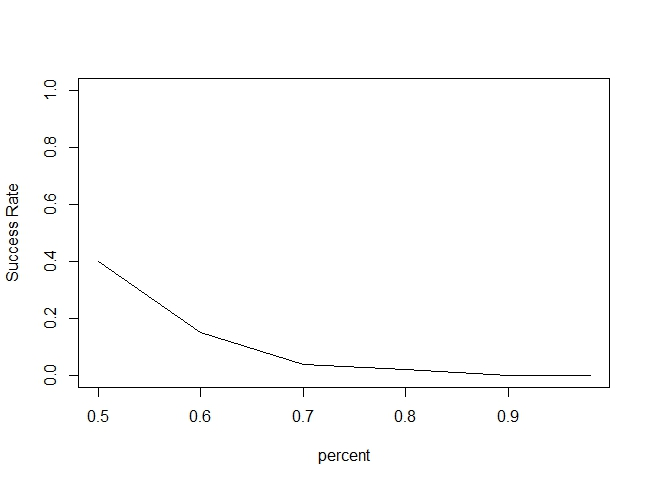
\includegraphics[scale=0.5]{Images/plot_smallC.jpeg}
\end{center} 
\vspace{2mm}
We now notice that the success rate is lower than the paper suggests, but there are many reasons for this. First, we are not analyzing the same corpus. Second, LDA uses Variational EM methods to fit the topic distribution, which is a stochastic process. Even though the overall success rate is lower, the trend stays the same. LDA tends to produce the correct generative model when the percentage of English documents is lower. In this example, when the percentage of English documents is greater than $0.9$, LDA never produces the generative model.

\subsection{TopicMapping}

The second part of the paper introduces a new algorithm for topic modeling called TopicMapping. The algorithm is described in \cite{main}, with more details in \cite{mainExtra}. In order to reproduce the article's main empirical results, I need to run their algorithm. I contacted the author's to not only obtain their original data, but their code if possible. I received code from one of the authors. The code is written mostly in C++, but also in Python. After several attempts, I was able to successfully run their code on a mac, but have run into the following error on a pc:  ``InfoMap did not compile. Please contact me: arg.lanci@gmail.com ." I have sent an email asking for help, but have yet to hear back. I was also able to code the algorithm in R. However, my code is neither efficient nor fast. For the following results, I ran everything I could on my pc, but decided to simply run the TopicMapping algorithm on a mac, save the results to a flash drive, and upload them to my pc for analysis. 

\subsection{Comparison of LDA to TopicMapping}

There are two types of major synthetic data analyzed in the paper. The first type of data is similar to that in Section 2.1, with corpuses of differing sizes contain ten languages in different proportions. The other type of data consists of corpuses constructed using the generative process defined in \cite{lda}, where the number of documents is $1000,$ the number of words in each document is $50$, the number of topics is set to $20$, and the hyper-parameters are set at $\alpha=0.001,0.004,0.016,0.064$. They also vary the percentage of words in the corpus that are considered generic, or equally likely across topics. Along with considering cases where each topic is equally distributed across documents, they consider cases where four topics make up $15\%$ and the last $16$ topics make up $2.5\%$. To simplify the amount of computing, I will focus on six corpuses of the first type:  Three corpuses have ten equally distributed languages of size $1000, 5000, 10000,$ and the other three have two languages making up $15\%$ each of the corpus and the remaining eight languages making up $8.75\%$ of size $1000, 5000, 10000$. I will also analyze twelve corpuses of the second type:  Six corpuses have $\alpha=0.001$ with generic proportion $0.2, 0.5, 0.8,$ and either equal topic distribution or not; the last six have $\alpha=0.064$ with generic proportion $0.2, 0.5, 0.8$, and either equal topic distribution or not.
\\

\noindent I was able to compile the code given to me by the authors, which simulate similar, but not the exact synthetic datasets. They did not save their original seed values. I was also able to successfully compile their program, which calculates the accuracy and reproducibility of a model. My aim is to reproduce the results as shown in Fig. 4 (pg.5, \cite{main}) and Fig. 7 (pg.6, \cite{main}) using a mac to run the TopicMapping algorithm and my pc to run LDA in R. The two other models that are considered by the authors are pLSA and LDA with seeded start values. Since the authors do not provide an explanation of what the start seeds are or how to find them, I ignore this model comparison. I also ignore the comparison to pLSA since this algorithm is not already programed in R nor do the authors provide code for it. The results for LDA and pLSA were similar to the results of LDA in all cases studies considered. Therefore, I will focus on reproducing the results for comparisons between TopicMapping and randomly seeded symmetric LDA only.
\\

\noindent I begin with the language corpuses, where I obtained the following accuracy and reproducibility results:
\vspace{2mm}
\begin{center}
	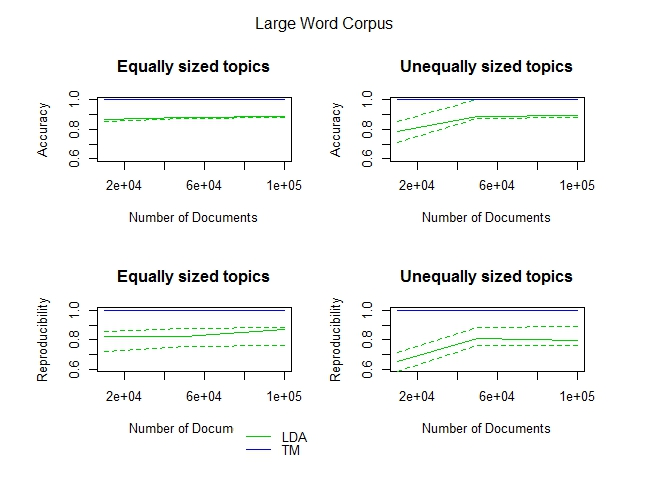
\includegraphics[scale=0.7]{Images/plot_largeC.jpeg}
\end{center} 
\vspace{2mm}
\noindent The plot above shows accuracy (top) and reproducibility (bottom) results for running LDA (green) and TopicMapping (blue) $100$ times on both equal (left) and unequal (right) topic distributions. With both algorithms, the number of topics was fixed at $10$. The median for the $100$ runs is plotted, where dotted lines indicate the $25$th and $75$th percentiles for both algorithms as described in \cite{main}. We can clearly see that the results follow the same patterns as shown in \cite{main}. TopicMapping is performing at near perfect accuracy and reproducibility for both equally and unequally sized topics regardless of the number of documents in the corpus. LDA clearly performs with greater variance, and does slightly better as the number of documents increases. Yet, TopicMapping outperforms LDA in all cases.
\\

\noindent The next results we will look at are those obtained from running both LDA and TopicMapping on the second set of simulated datasets when the hyper-parameters are set to $0.001$:
\vspace{2mm}
\begin{center}
	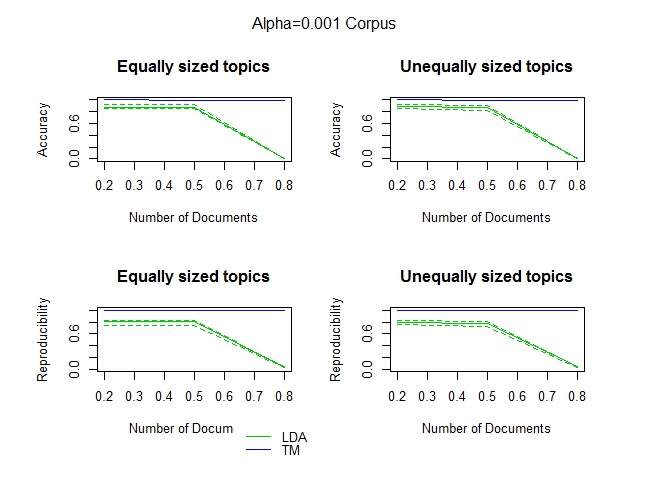
\includegraphics[scale=0.8]{Images/plot_Alpha1.jpeg}
\end{center} 
\vspace{2mm}

\noindent The figure above shows accuracy (top) and reproducibility (bottom) results for running LDA (green) and TopicMapping (blue) $100$ times on both equal (left) and unequal (right) topic distributions. With both algorithms, the number of topics was fixed at $20$ and the hyper-parameters are set at $0.001$. Again, the median for $100$ runs is plotted, where dotted lines indicate the $25$th and $75$th percentiles for both algorithms. We can clearly see that the results follow the same patterns as shown in \cite{main}. TopicMapping is performing at near perfect accuracy and reproducibility for both equally and unequally sized topics regardless of the number of documents in the corpus. LDA clearly performs with greater variance, and does slightly better as the percentage of generic words decreases. Yet, TopicMapping outperforms LDA in all cases.
\\

\noindent Lastly, we will look at the results obtained from running both LDA and TopicMapping on the second set of simulated datasets when the hyper-parameters are set to $0.064$:
\vspace{2mm}
\begin{center}
	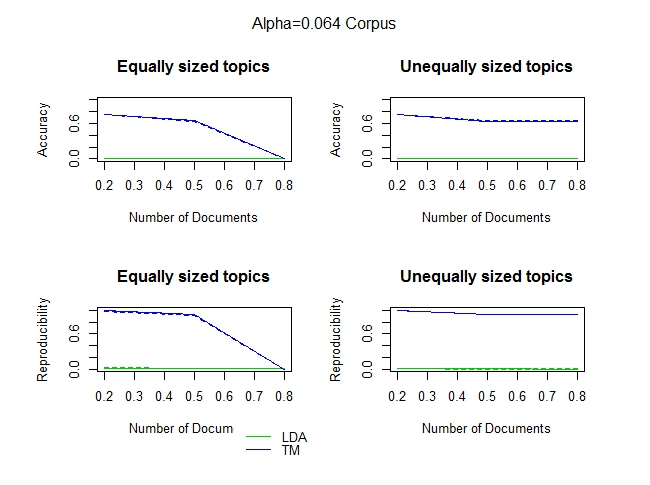
\includegraphics[scale=0.7]{Images/plot_Alpha2.jpeg}
\end{center} 
\vspace{2mm}

\noindent The figure above shows accuracy (top) and reproducibility (bottom) results for running LDA (green) and TopicMapping (blue) $100$ times on both equal (left) and unequal (right) topic distributions. With both algorithms, the number of topics was fixed at $20$ and the hyper-parameters are set at $0.064$. Again, the median for $100$ runs is plotted, where dotted lines indicate the $25$th and $75$th percentiles for both algorithms. We can clearly see that the results follow similar patterns as shown in \cite{main}. Both LDA and TopicMapping perform uniformly across differing percentages of generic words. TopicMapping with $0.7$ accuracy and $0.8$ reproducibility outperforms LDA, which performs poorly. Although LDA consistently performs poorly with unequally sized topics, TopicMapping's accuracy and reproducibility drop as the percentage of generic words increases, which is exactly what we see in \cite{main}.


\subsection{Applications}

I received emails back from two of the authors providing me with the corpus for the first application dataset:  \textit{Web of Science} or WoS. Both authors stated that the second application dataset, Wikipedia, was too large to send. They stated that even if they provided me access to it through some means, I would be unable to successfully reproduce their results in a semester. I will focus on reproducing the results for the first application only. The WoS Corpus contains documents consisting of the titles and abstracts for $23838$ journal articles published in six different top journals for the following fields:  astronomy, biology, economics, geology, mathematics, and psychology. I was able to reproduce the results on Fig. 8 (pg. 7, \cite{main}):

\vspace{2mm}
\begin{center} 
	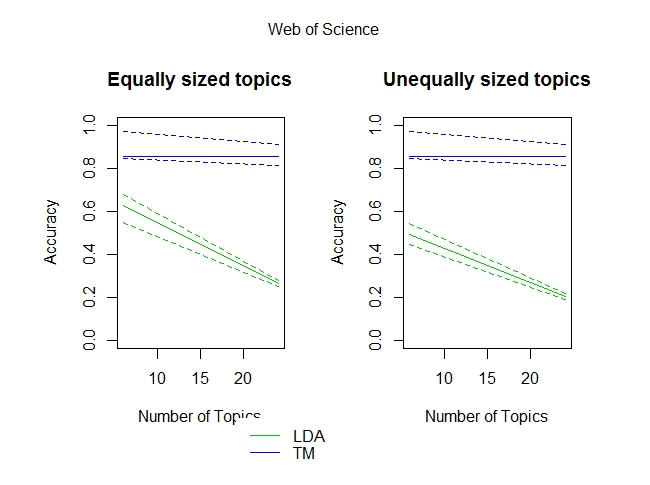
\includegraphics[scale=0.4]{Images/plot_WoS.jpeg} 
\end{center} 
\vspace{2mm}  

\noindent I have plotted the median accuracy (left) and reproducibility (right) from the $100$ runs for both TopicMapping (blue) and LDA (green) with dotted lines representing the $25$th and $75$th percentiles. The results were found when the number of topics was set at $6$ the correct number and at $24$ as in \cite{main}. We notice that with both cases the correct number of topics and incorrect number, TopicMapping does well in both accuracy and reproducibility. However, LDA performs better when the correct number of topics specified. Again, TopicMapping outperforms LDA in all cases. 

\newpage
\hypertarget{B}{}
\section{ERGM GOF}
From the MCMC diagnostics plots below, we can see that the MCMC estimates converged:
\vspace{2mm}
\begin{center} 
	%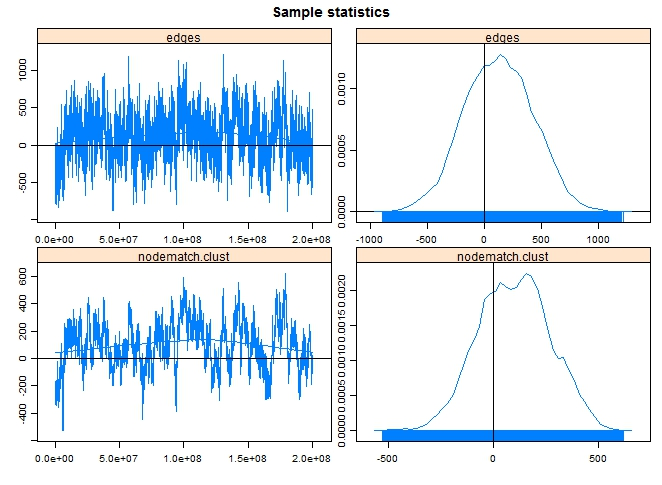
\includegraphics[scale=0.4]{Images/sci_mcmc1.jpeg} 
	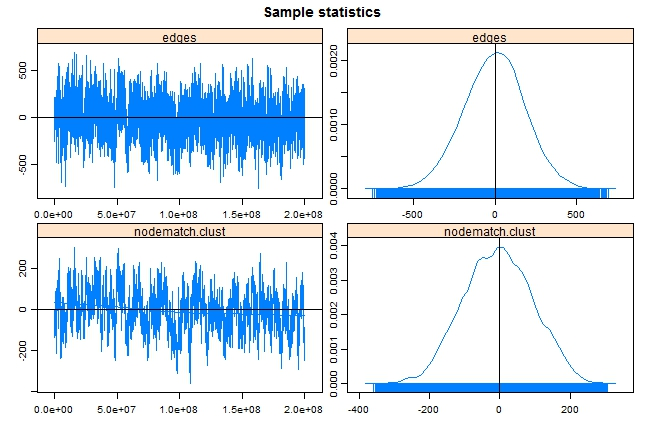
\includegraphics[scale=0.4]{Images/ind_mcmc1.jpeg} 
\end{center} 
\vspace{2mm}
The Geweke statistics for the Science and Indeed corpus were all insignificant at the 0.05 level with an overall p-value of 0.1125 and 0.04224, respectively. The quantiles can be seen below:
 \vspace{2mm}
 \begin{center}
 	\begin{tabular}{ |c||c|c|c|c|c|  }
 		\hline
 		&$2.5\%$     &$25\%$     &$50\%$    &$75\%$  &$97.5\%$ \\
 		\hline
 		Science&&&&& \\
 		\hline
 		edges&           -387&  -154&  -24&  106&  363 \\
 		nodematch.clust&  -247&  -103&  -22&  63&225 \\
 		\hline
 		Indeed&&&&& \\
 		\hline
 		edges&           -376&  -131&  -2&  121&  359 \\
 		nodematch.clust&  -191&  -73&  -5&  64&183 \\
 		\hline
 	\end{tabular}
 \end{center}
 \vspace{2mm}
We can clearly see that both ergms are not degenerate. However in the following goodness of fit plots, we can see how complex these networks are. Neither ergm fits the data well:
\vspace{2mm}
\begin{center} 
	
\includegraphics[scale=0.05]{Images/Sci_fit2.pdf} 
	
\includegraphics[scale=0.05]{Images/Indeed_fit2.pdf} 
\end{center} 
\vspace{2mm}
The following show the first part of each image blown up. We can now clearly see that neither ergm model fits well:
\vspace{2mm}
\begin{center} 
	
\includegraphics[scale=0.5]{Images/Sci_fit2.pdf} 
	
\includegraphics[scale=0.5]{Images/Indeed_fit2.pdf} 
\end{center} 
\vspace{2mm}


\end{document}